\section{Actores}

Los actores que interactúan con el sistema se visualizan en la Figura \ref{fig:actoresTASMC}.

\begin{table}[htbp]
	\begin{center}
		\begin{tabular}{|p{2.5cm}|p{6.4cm}|p{2cm}|p{2cm}|}
			\hline
				\rowcolor[RGB]{255,102,102}{Actor}&\multicolumn{2}{c}{Usuario}&{\textbf{ACT-01}}\\
			\hline
				{Descripción}&\multicolumn{3}{p{11.2cm}|}{
			Es el actor principal y por lo tanto tiene la mayor interacción con el sistema. El usuario hace uso de todos 				los servicios proporcionados por la aplicación, es decir, configuración de viaje dependiendo de gustos y 					posibilidades, consultar sugerencias de vuelos y hoteles, control de equipaje, uso de itinerario de viaje, la 				creación de ruta óptima casa-aeropuerto, localización dentro del AICM y visualizar estado de vuelo.}\\
			\hline
				{Características}&\multicolumn{3}{p{11.2cm}|}{Actor Primario}\\
			\hline
				{Referencias}&\multicolumn{3}{p{11.2cm}|}{Caso de Uso General}\\
			\hline
				{Autor}&{Vivanco Carmona Erick Rafael}&{\textbf{Fecha} 09/01/15}&{\textbf{Versión} 2.0}\\
			\hline
				{Evaluador}&{Barajas Uribe Sergio}&{\textbf{Fecha} 15/01/15}&{\textbf{Estatus} Aprobado}\\
			\hline
				{Comentarios}&\multicolumn{3}{p{11.2cm}|}{Al ser el actor principal, la funcionalidad de la aplicación 						únicamente cobra sentido cuando el usuario inicia la aplicación y hace uso de los servicios 										proporcionados por el sistema.}\\
			\hline
		\end{tabular}
	\end{center}
	\caption[Descripción del Perfil del Actor Usuario]{Descripción del Perfil del Actor Usuario}
    	\label{tab:perfilUsuario}
\end{table}

\begin{figure}[htbp]
	\centering
		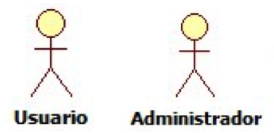
\includegraphics[width=0.5\textwidth]{Figuras/actores.png}
		\rule{30em}{0.5pt}
	\caption[Actores de TASMC]{Actores de TASMC}
	\label{fig:actoresTASMC}
\end{figure}

\begin{table}[htbp]
	\begin{center}
		\begin{tabular}{|p{2.5cm}|p{6.4cm}|p{2cm}|p{2cm}|}
			\hline
				\rowcolor[RGB]{255,102,102}{Actor}&\multicolumn{2}{c}{Administrador}&{\textbf{ACT-02}}\\
			\hline
				{Descripción}&\multicolumn{3}{p{11.2cm}|}{
			Es el encargado de gestionar los elementos de hardware y software del sistema (Base de datos, Servidor y Web Service).}\\
			\hline
				{Características}&\multicolumn{3}{p{11.2cm}|}{Actor Secundario}\\
			\hline
				{Referencias}&\multicolumn{3}{p{11.2cm}|}{Caso de Uso General}\\
			\hline
				{Autor}&{Vivanco Carmona Erick Rafael}&{\textbf{Fecha} 09/01/15}&{\textbf{Versión} 2.0}\\
			\hline
				{Evaluador}&{Barajas Uribe Sergio}&{\textbf{Fecha} 15/01/15}&{\textbf{Estatus} Aprobado}\\
			\hline
				{Comentarios}&\multicolumn{3}{p{11.2cm}|}{Sin la gestión que realiza este actor al sistema no puede dar la funcionalidad necesaria para proporcionar al usuario los beneficios de la aplicación.}\\
			\hline
		\end{tabular}
	\end{center}
	\caption[Descripción del Perfil del Actor Administrador]{Descripción del Perfil del Actor Administrador}
    	\label{tab:perfilAdministrador}
\end{table}